% **************************************************************************************************
% ** SPSC Report and Thesis Template
% **************************************************************************************************

\newcommand{\DocumentType}{report} % "thesis" / "report" / "homework"
\newcommand{\DocumentLanguage}{en} % "en" / "de"
\newcommand{\PaperSize}{a4paper} % "a4paper" / "letterpaper"
\newcommand{\Twosided}{false} % "true" / "false"

% **************************************************************************************************
% template setup -- do not change these unless you know what you are doing!
\input{./base/packages_\DocumentType}
\input{./base/layout_\DocumentType}
% **************************************************************************************************
% ** SPSC Report and Thesis Template
% **************************************************************************************************
%
% ***** Authors *****
% Daniel Arnitz, Paul Meissner, Stefan Petrik
% Signal Processing and Speech Communication Laboratory (SPSC)
% Graz University of Technology (TU Graz), Austria
%
% ***** Changelog *****
% 0.1   2010-08-09   added \remc and \remq commands, \nxtpar now uses \med- instead of \bigskip
%                    replaced \lastfootnotemark by \oldfootnotemark (generalization),
%                    added \chapternote, set \openingquote to 0.4\textwidth, modified \MAttention,
%                    \xspace for marginpar commands, modified \MDanger and \MQuestion
% 0.2   2010-10-03   added \exp, colors "bk*"
% 0.3   2010-11-16   added \twofigs and \twofigsf
% 0.4   2010-12      added \F (Fourier), \ceil and \floor
% 0.5   2011-01      added chapter/section/figure/table/part reference commands, textrel
% 0.6   2011-03      added \avg, modified bkred, bkgreen, and bkblue colors,
%                    added \medskip to \chapternote, added natural/real/complex/... numbers
%                    added \rapp for references to the appendix
% 0.7   2011-04      removed labels from \new*NoTOC
% 0.8   2012-06      correction of minor typo
% 0.9   2013-01      fixed parentheses in \openingquote (bug reported by Angelika Kern)
%
% ***** Todo *****
% ? prettyref instead of reference commands
%
% **************************************************************************************************



% **************************************************************************************************
% * SECTIONING AND TEXT
% **************************************************************************************************

% new chapter, section, ... plus a few addons
%   part
\newcommand{\newpart}[2]{\FloatBarrier\cleardoublepage\part{#1}\label{part:#2}}%
%   chapter
\newcommand{\newchapter}[2]{\FloatBarrier\chapter{#1}\label{chp:#2}}
\newcommand{\newchapterNoTOC}[1]{\FloatBarrier\stepcounter{chapter}\chapter*{#1}}%
%   section
\newcommand{\newsection}[2]{\FloatBarrier\vspace{5mm}\section{#1}\label{sec:#2}}%
\newcommand{\newsectionNoTOC}[1]{\FloatBarrier\vspace{5mm}\stepcounter{section}\section*{#1}}%
%   subsection
\newcommand{\newsubsection}[2]{\FloatBarrier\vspace{3mm}\subsection{#1}\label{sec:#2}}%
\newcommand{\newsubsectionNoTOC}[1]{\FloatBarrier\vspace{3mm}\stepcounter{subsection}\subsection*{#1}}%
%   subsubsection
\newcommand{\newsubsubsection}[2]{\vspace{2mm}\subsubsection{#1}\label{sec:#2}}%
\newcommand{\newsubsubsectionNoTOC}[1]{\vspace{2mm}\stepcounter{subsubsection}\subsubsection*{#1}}%

% references
%   chapter(s), section(s), appendix
\newcommand{\rchp}[1]{Chapter~\ref{chp:#1}}
\newcommand{\rchps}[1]{Chapters~\ref{chp:#1}}
\newcommand{\rsec}[1]{Section~\ref{sec:#1}}
\newcommand{\rsecs}[1]{Sections~\ref{sec:#1}}
\newcommand{\rappendix}[1]{Appendix~\ref{#1}}
%   figure(s), table(s), listing(s), equation(s)
\newcommand{\rfig}[1]{Fig.~\ref{fig:#1}}
\newcommand{\rfigs}[1]{Figs.~\ref{fig:#1}}
\newcommand{\rtab}[1]{Tab.~\ref{tab:#1}}
\newcommand{\rtabs}[1]{Tabs.~\ref{tab:#1}}
\newcommand{\rlst}[1]{Listing~\ref{lst:#1}}
\newcommand{\rlsts}[1]{Listings.~\ref{lst:#1}}
\newcommand{\req}[1]{(\ref{eq:#1})}

% varioref references
%   chapter(s), section(s)
\newcommand{\vrchp}[1]{Chapter~\vref{chp:#1}}
\newcommand{\vrchps}[1]{Chapters~\vref{chp:#1}}
\newcommand{\vrsec}[1]{Section~\vref{sec:#1}}
\newcommand{\vrsecs}[1]{Sections~\vref{sec:#1}}
%   figure(s), table(s), listing(s)
\newcommand{\vrfig}[1]{Fig.~\vref{fig:#1}}
\newcommand{\vrfigs}[1]{Figs.~\vref{fig:#1}}
\newcommand{\vrtab}[1]{Tab.~\vref{tab:#1}}
\newcommand{\vrtabs}[1]{Tabs.~\vref{tab:#1}}
\newcommand{\vrlst}[1]{Listing~\vref{lst:#1}}
\newcommand{\vrlsts}[1]{Listings~\vref{lst:#1}}

% next paragraph
\newcommand{\nxtpar}{\par\medskip}

% "stylish" quotes on the right side
\ifthenelse{\equal{\DocumentLanguage}{en}}{\newcommand{\openingquote}[2]{\hfill\parbox[t]{10cm}{\itshape\raggedleft{``#1''}\\\footnotesize -- #2}\nxtpar}}{}%
\ifthenelse{\equal{\DocumentLanguage}{de}}{\newcommand{\openingquote}[2]{\hfill\parbox[t]{10cm}{\itshape\raggedleft{"`#1"'}\\\footnotesize -- #2}\nxtpar}}{}%

% some information on the right side (sources, ...)
\newcommand{\chapternote}[1]{\vspace*{-\medskipamount}\hfill\parbox[t]{0.8\textwidth}{\itshape\footnotesize\raggedleft#1}\par\medskip}%

% direct quotes
% \newenvironment{directquote}{\nxtpar\hrule}{\hrule}\hfill\litref{#1}{#2}}

% warnings and attention signs in marginpar
\newcommand{\MDanger}{\marginpar{\raisebox{-2mm}{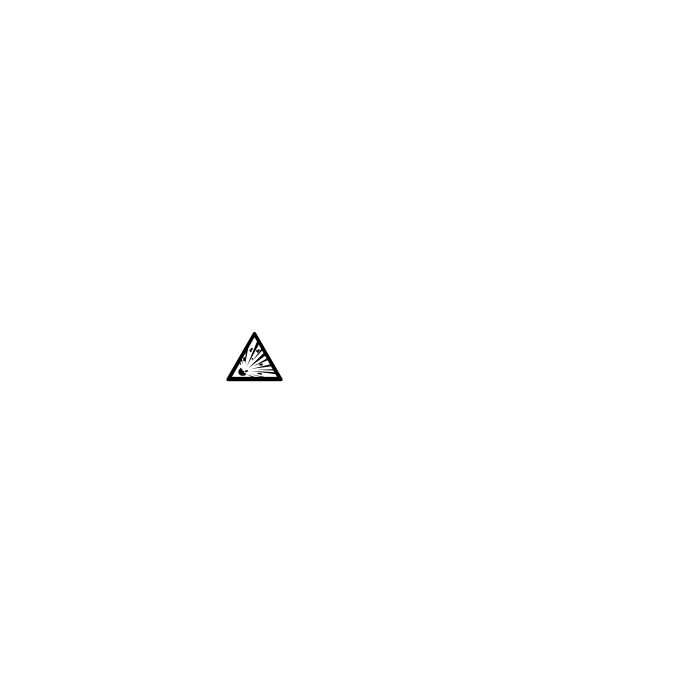
\includegraphics[height=7mm]{base/MDanger}}}\xspace}%
\newcommand{\MAttention}{\marginpar{\raisebox{-2mm}{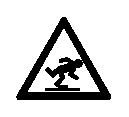
\includegraphics[height=7mm]{base/MAttention}}}\xspace}%
\newcommand{\MHint}{\marginpar{\raisebox{-2.25mm}{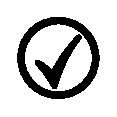
\includegraphics[height=7mm]{base/MHint}}}\xspace}%
\newcommand{\MQuestion}{\marginpar{\raisebox{-2.25mm}{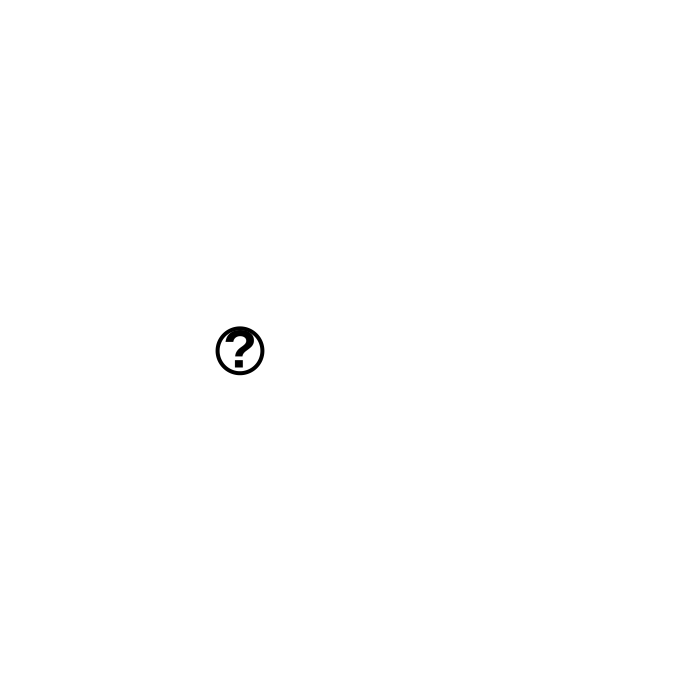
\includegraphics[height=7mm]{base/MQuestion}}}\xspace}%

% same footnote number as last one
\newcommand{\oldfootnotemark}[1]{\addtocounter{footnote}{-#1}\footnotemark\addtocounter{footnote}{#1-1}}%
%\newcommand{\lastfootnotemark}{\addtocounter{footnote}{-1}\footnotemark}%

% value-unit commands (for 457 kHz, etc)
\newcommand{\vu}[2]{\mbox{\ensuremath{#1\,\text{#2}}}}% "value-unit" ... prevents e.g. 456 \linebreak mV
\newcommand{\vuc}[3]{\mbox{\ensuremath{#1\,\text{#2}\;#3\,\%}}} % "value~unit~tolerance-per-cent"
\newcommand{\vum}[3]{\mbox{\ensuremath{#1\,\text{#2}\;#3\,\perthousand}}} % "value~unit~tolerance-per-mil"

% reminders
\newcommand{\reminder}[1]{\colorbox{red}{#1}\xspace}%
\newcommand{\rem}{\reminder{(...)}}% shortcut for the full reminder
\newcommand{\remq}{\reminder{???}}% open question
\newcommand{\remc}{\reminder{[?]}}% open citation
\newcommand{\uc}{\nxtpar\colorbox{yellow}{... under construction ...}\nxtpar}%

% misc
\newcommand{\pwd}{.} % present working directory (can be used to create relativ paths per part, etc.)




% **************************************************************************************************
% * MATH
% **************************************************************************************************

% highlighting
\newcommand{\vm}[1]{\ensuremath{\bm{#1}}}% vector or matrix

% functions
\renewcommand{\exp}[1]{\ensuremath{\text{e}^{#1}}}% exponential
\renewcommand{\ln}[1]{\ensuremath{\text{ln}\!\left(#1\right)}}% natural logarithm
\newcommand{\ld}[1]{\ensuremath{\text{ld}\!\left(#1\right)}}% logarithm base 2
\renewcommand{\log}[1]{\ensuremath{\text{log}\!\left(#1\right)}}% logarithm (base 10)
\newcommand{\logb}[2]{\ensuremath{\text{log}_{#1}\!\left(#2\right)}}% logarithm base ...

% rounding
\newcommand{\round}[1]{\ensuremath{\text{round}\!\left(#1\right)}}% rounding towards next integer
\newcommand{\ceil}[1]{\ensuremath{\left\lceil#1\right\rceil}}% rounding towards infinity
\newcommand{\floor}[1]{\ensuremath{\left\lfloor#1\right\rfloor}}% rounding towards zero

% operators
\newcommand{\E}[1]{\ensuremath{\text{E}\!\left\{#1\right\}}}% expectation operator
\newcommand{\F}[1]{\ensuremath{\mathcal{F}\!\left\{#1\right\}}}% Fourier transform operator
\newcommand{\IF}[1]{\ensuremath{\mathcal{F}^{-1}\!\left\{#1\right\}}}% inverse Fourier transform operator
\newcommand{\var}[1]{\ensuremath{\text{var}\!\left\{#1\right\}}}% variance operator
\newcommand{\cov}[1]{\ensuremath{\text{cov}\!\left\{#1\right\}}}% covariance operator
\newcommand{\corr}[1]{\ensuremath{\text{corr}\!\left\{#1\right\}}}% correlation operator
\newcommand{\avg}[1]{\ensuremath{\text{avg}\!\left\{#1\right\}}}% averaging operator
\newcommand{\avgvar}[1]{\ensuremath{\overline{\text{var}}\!\left\{#1\right\}}}% average variance operator
\renewcommand{\Re}[1]{\ensuremath{\text{Re}\!\left\{#1\right\}}}% real part
\renewcommand{\Im}[1]{\ensuremath{\text{Im}\!\left\{#1\right\}}}% imaginary part

% numbers
\newcommand{\REAL}{\ensuremath{\mathbb{R}}}% real numbers
\newcommand{\NATURAL}{\ensuremath{\mathbb{N}}}% natural numbers
\newcommand{\INTEGER}{\ensuremath{\mathbb{Z}}}% integer numbers (natural numbers plus zero)
\newcommand{\COMPLEX}{\ensuremath{\mathbb{C}}}% complex numbers
\newcommand{\IMAG}{\ensuremath{\mathbb{I}}}% imaginary numbers

% other
\newcommand{\conj}{\ensuremath{^\ast}}% conjugate complex
\newcommand{\transp}{\ensuremath{^\text{T}}}% conjugate (Hermitian) transpose
\newcommand{\mtx}[2]{\left[\ensuremath{\begin{array}{#1}#2\end{array}\right]}}%vector/matrix
\newcommand{\isdef}{\ensuremath{\mathrel{:=}}}% definition left->right
\newcommand{\isdefflip}{\ensuremath{\mathrel{=:}}}% definition right->left
\newcommand{\isreq}{\ensuremath{\mathrel{\stackrel{!}{=}}}}% is required
\newcommand{\textrel}[1]{\ensuremath{{\;{#1}\;}}}% relation symbol for in-line equations (fixed spacing)



% **************************************************************************************************
% * FLOATS (FIGURES, TABLES, LISTINGS, ...)
% **************************************************************************************************

% figures without frames
%   standard
\newcommand{\fig}[3]{\begin{figure}\centering\includegraphics[width=\textwidth]{#1}\caption{#2}\label{fig:#3}\end{figure}}%
%   with controllable parameters
\newcommand{\figc}[4]{\begin{figure}\centering\includegraphics[#1]{#2}\caption{#3}\label{fig:#4}\end{figure}}%
%   two subfigures
\newcommand{\twofig}[6]{\begin{figure}\centering%
\subfigure[#2]{\includegraphics[width=0.495\textwidth]{#1}}%
\subfigure[#4]{\includegraphics[width=0.495\textwidth]{#3}}%
\caption{#5}\label{fig:#6}\end{figure}}%
%   two subfigures with labels for each subplot
\newcommand{\twofigs}[8]{\begin{figure}\centering%
\subfigure[#2]{\includegraphics[width=0.495\textwidth]{#1}\label{fig:#8#3}}%
\subfigure[#5]{\includegraphics[width=0.495\textwidth]{#4}\label{fig:#8#6}}%
\caption{#7}\label{fig:#8}\end{figure}}%
%   two subfigures and controllable parameters
\newcommand{\twofigc}[8]{\begin{figure}\centering%
\subfigure[#3]{\includegraphics[#1]{#2}}%
\subfigure[#6]{\includegraphics[#4]{#5}}%
\caption{#7}\label{fig:#8}\end{figure}}%

% framed figures
%   standard
\newcommand{\figf}[3]{\begin{figure}\centering\fbox{\includegraphics[width=\textwidth]{#1}}\caption{#2}\label{fig:#3}\end{figure}}%
%   with controllable parameters
\newcommand{\figcf}[4]{\begin{figure}\centering\fbox{\includegraphics[#1]{#2}}\caption{#3}\label{fig:#4}\end{figure}}%
%   two subfigures
\newcommand{\twofigf}[6]{\begin{figure}\centering%
\fbox{\subfigure[#2]{\includegraphics[width=0.495\textwidth]{#1}}}%
\fbox{\subfigure[#4]{\includegraphics[width=0.495\textwidth]{#3}}}%
\caption{#5}\label{fig:#6}\end{figure}}%
%   two subfigures with labels for each subplot
\newcommand{\twofigsf}[8]{\begin{figure}\centering%
\fbox{\subfigure[#2]{\includegraphics[width=0.495\textwidth]{#1}\label{fig:#8#3}}}%
\fbox{\subfigure[#5]{\includegraphics[width=0.495\textwidth]{#4}\label{fig:#8#6}}}%
\caption{#7}\label{fig:#8}\end{figure}}%
%   two subfigures and controllable parameters
\newcommand{\twofigcf}[8]{\begin{figure}\centering%
\fbox{\subfigure[#3]{\includegraphics[#1]{#2}}}%
\fbox{\subfigure[#6]{\includegraphics[#4]{#5}}}%
\caption{#7}\label{fig:#8}\end{figure}}%

% listings
\newcommand{\filelisting}[4]{\lstinputlisting[print=true,language=#1,caption={#3},label={lst:#4}]{#2}}

% preserve backslash for linebreaks in tables (ragged... redefines \\, thus it has to be preserved)
\newcommand{\pbs}[1]{\let\temp=\\#1\let\\=\temp}%


% **************************************************************************************************
% * MISC
% **************************************************************************************************

% slighly darkened colors for text
\definecolor{bkred}{rgb}{0.9,0,0}
\definecolor{bkgreen}{rgb}{0,0.67,0}
\definecolor{bkblue}{rgb}{0,0,0.75}
\definecolor{mygreen}{rgb}{0,0.6,0}
\definecolor{mygray}{rgb}{0.5,0.5,0.5}
\definecolor{mymauve}{rgb}{0.58,0,0.82}
% \graphicspath{{./drawings/}{./plots/}{./images/}}
% **************************************************************************************************
% ATTENTION: There is a stylesheet provided for makeindex; set makeindex to -s "./base/index.sty"
% **************************************************************************************************

% uncomment to get watermarks:
% \usepackage[first,bottom,light,draft]{draftcopy}
% \draftcopyName{ENTWURF}{160}


% **************************************************************************************************
% information fields

% general
\newcommand{\DocumentTitle}{Driver Development}
\newcommand{\DocumentSubtitle}{Linux Module \newline for the RFM12 on the Xilinx MicroZed Board}
\newcommand{\ShortTitle}{RFM12} % used in headers (keep short!)
\newcommand{\DocumentAuthor}{ Armin Schönlieb}
\newcommand{\DocumentDate}{Graz, \today}
%    for thesis only (will be ignored for reports)
\newcommand{\ThesisType}{module Report}
\newcommand{\Supervisors}{Adrian Remonda} % Supervisor 1 \\ Supervisor 2 \\ ...
%   for report only: revision number
\newcommand{\RevPrefix}{alpha~}
\newcommand{\RevLarge}{1}
\newcommand{\RevSmall}{0}

% confidential? (can of course also be used for other messages/notes)
\newcommand{\ConfidNote}{\textbf{RFM12 Module}, \today}

% correct bad hyphenation
\hyphenation{}
% **************************************************************************************************
% ** SPSC Report and Thesis Template
% **************************************************************************************************
%
% ***** Authors *****
% Daniel Arnitz, Paul Meissner, Stefan Petrik
% Signal Processing and Speech Communication Laboratory (SPSC)
% Graz University of Technology (TU Graz), Austria
%
% ***** Changelog *****
% 0.1   2012-07-20   \OptDraft and \ContentBox
%
% ***** Todo *****
%
% **************************************************************************************************


% optional boxes with intended contents or other comments (can be switched on/off)
\newcommand{\ContentBox}[2]{\ifthenelse{\boolean{DisplayContentBoxes}}{\FloatBarrier\nxtpar\colorbox{yellow}{\parbox{\textwidth}{\footnotesize#1\par\hrulefill\par Number of pages: #2}}\nxtpar}{}}

% optional draft mode for large graphics (add \OptDraft to parameters for \includegraphics)
%\ifthenelse{\boolean{OptDraftMode}}{\newcommand{\OptDraft}{draft}}{\newcommand{\OptDraft}{keepaspectratio}}

\usepackage{listings}
\renewcommand{\lstlistingname}{Code}
\lstset{
   basicstyle=\scriptsize\ttfamily,
   keywordstyle=\color{blue},
   stringstyle=\color{mygreen},
   commentstyle=\color{mygreen},
   emph={square}, 
   emphstyle=\color{mymauve},
   tabsize=2,
	 showstringspaces=false,
   flexiblecolumns=false,
   numbers=left,
   numberstyle=\tiny\color{mygray},
   stepnumber=1,
   numbersep=5pt,
   xleftmargin=15pt,
	 language=C++,
	 captionpos=t
 }


% **************************************************************************************************
% **************************************************************************************************
% **************************************************************************************************
\begin{document}
% **************************************************************************************************
% titlepage
\input{./base/titlepage_\DocumentType}\emptydoublepage
%\emptydoublepage
\tableofcontents

% **************************************************************************************************
% mainmatter\color[rgb]{0,0,0}
\chapter{Introduction}

The code for the whole Project can be found on GitHub via this Link \url{https://github.com/SchoAr/RFM12_Linux}

\section{RFM12}
The RFM12 is a small Radio-Transceiver. The used version is sending and receiving with 433Mhz. The problem with this RF-Module is that it is hardly available any more.\newline
The Data-sheet of the RFM12 can be accessed from here : \url{http://www.hoperf.com/upload/rf/RFM12.pdf}\newline
The Chip uses a frequency shift keying method for sending and receiving. Only a half-duplex communication can be acquired. The whole specification of the chip can be found in the Data sheet and are not discussed in detail.

\begin{figure}[H]
	\centering
		\includegraphics[width=1.00\textwidth]{picture/rfm12.png}
	\caption{RFM12 Chip Pinout}
	\label{fig:rfm12}
\end{figure}

The chip is used with an SPI interface for communication. With an interrupt the Chip indicates if the FIFO is empty in sending mode, or the FIFO received a Byte. Therefore the main program can sleep in receiving mode, until the Interrupt arrives. Also a Byte can be send and the program can do other stuff, until the FIFO is empty and an interrupt occurs.\newline

The Antenna of the Chip has to be designed by one own. The Chip gives a Antenna-pin and a proper Antenna has to be attached on this pin. Therefore the length of the Antenna has to be calculated with the following Formula.

\begin{equation}
	\lambda = \frac{c}{f} = \frac{3\cdot 10^{8}}{433 \cdot 10^{6}} =  692.7mm
\end{equation}

This is the length of a whole wave with the Frequency of 433MHz. Because the whole length is not necessary a $\frac{\lambda}{4}$ Antenna is used.
This is a length of 17,3cm. As a Antenna material a wire, standing up in the air, is used.

\section{Test System}

For a proper test System a receiver had to be chosen. This Board will receive the Messages from the MicroZed Board. I have choose the mbed from \url{mbed.org}. This Board allows a rapid prototyping and users can create specific Library for hardware. The used library for the RFM12 can be found with this link \url{http://developer.mbed.org/users/hajesusrodrigues/code/RFM12B/}\newline

This Library provides basic functions for sending and receiving. It also provides a function for encryption. This is very helpful for sending important data via the ISM Band. But there is a problem with the Library, it is designed for the RFM12B. There are only a few differences but they are important. \newline

\textbf{The First difference is that the RFm12B needs a pull-up Resistor on the PIN FSK/DATA/nFFS. Secondly a special sync byte is needed. This Byte is: 0xD4.}\newline 

Not every Pin of the RFM12 is used. The Used Pins are shown in the following schematic, also visible is the $10k\Omega$ pull-up Resistor.
\begin{figure}[H]
	\centering
		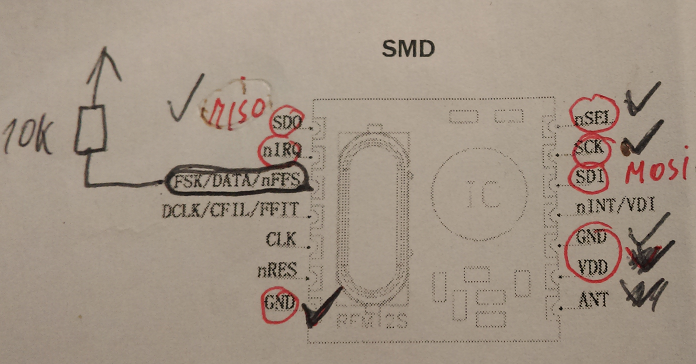
\includegraphics[width=1.00\textwidth]{picture/rfm12_connection.png}
	\caption{Pin out of the RFm12}
	\label{fig:rfm12_pinout}
\end{figure}

Not the real hardware with the Connections is shown in the following picture. One Connection is used as the required Pull up Resistor. The Antenna is not fully visible but standing up in the air.

\begin{figure}[H]
	\centering
		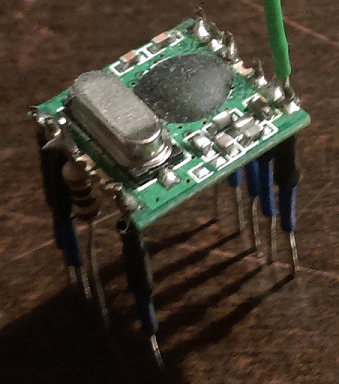
\includegraphics[width=1.00\textwidth]{picture/rfm12_connected.png}
	\caption{RFM12 Chip Connection Wired}
	\label{fig:rfm12_coonnection}
\end{figure}

The mbed test system is build-up on a bread board. The Following picture shows the Board: 

\begin{figure}[H]
	\centering
		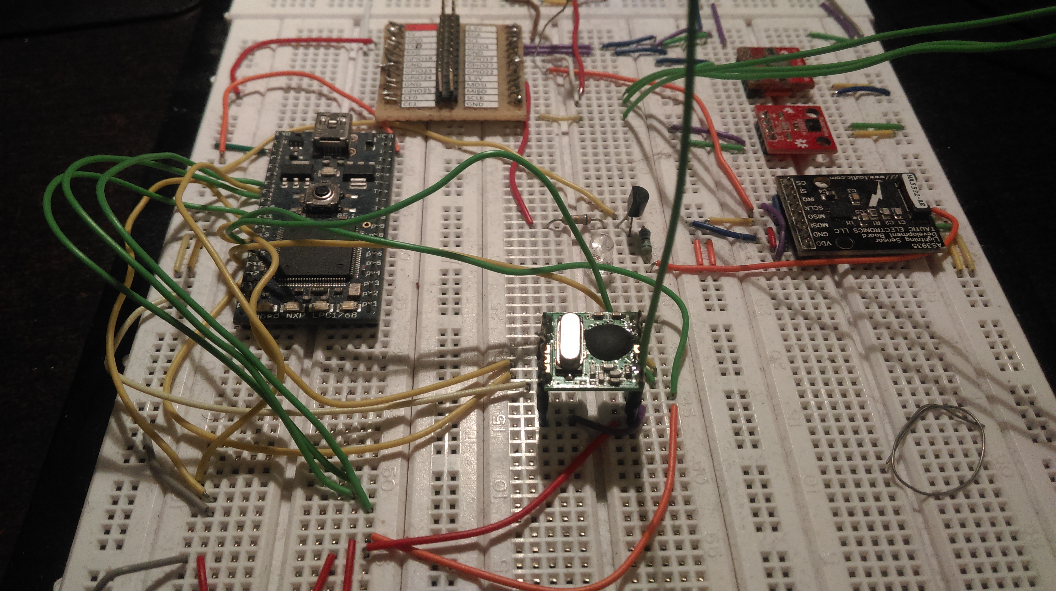
\includegraphics[width=1.00\textwidth]{picture/mbed_build.png}
	\caption{mbed test System}
	\label{fig:rfm12}
\end{figure}

For the connection with the MicroZed Board a special connection Board was Designed. It is a small Board providing the Connection with the RFM12 and 3 LEDs. The blue LED is designed for indicating that the Module is online, and the two green LEDs indicates receiving and transmitting. For Debugging a GND connection is available.

\begin{figure}[H]
	\centering
		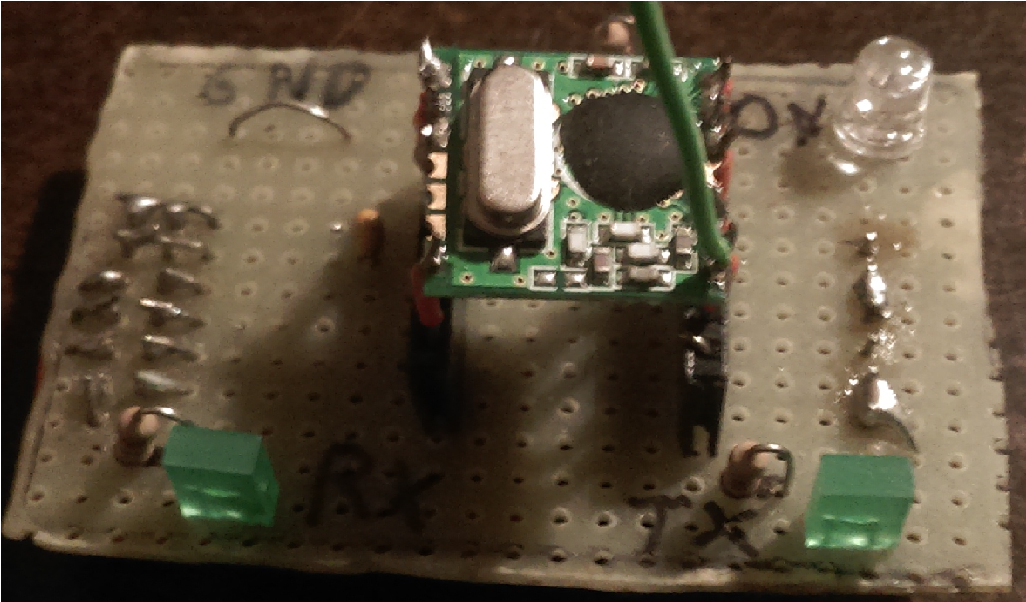
\includegraphics[width=1.00\textwidth]{picture/rfm12_carier.png}
	\caption{Carrier Board}
	\label{fig:rfm12}
\end{figure}

The Connection with the MicroZed Board is designed for the on-board connector. Because then no external Power supply is not required.

\begin{figure}[H]
	\centering
		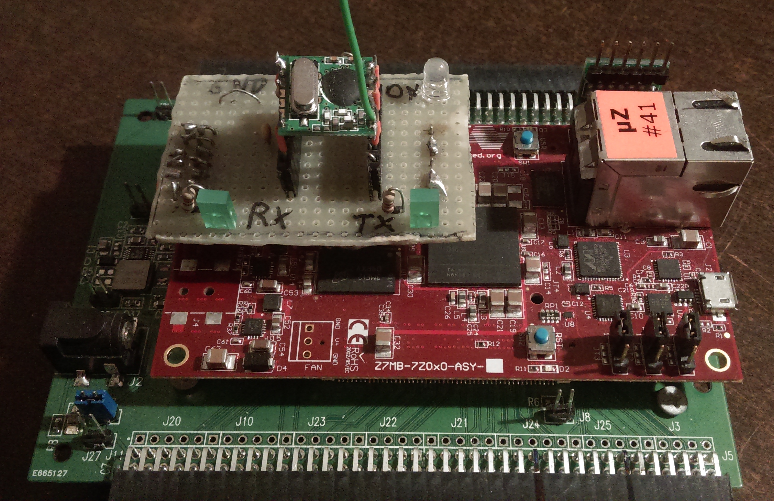
\includegraphics[width=1.00\textwidth]{picture/rfm12_carier_zynq.png}
	\caption{RFM12 connected to the MicroZed Board}
	\label{fig:rfm12}
\end{figure}

The Following table describes the Connection of the RFM12 Carrier board with the MicroZed Board.

\begin{table}[H]
    \centering
    \begin{tabular}{ c | c | c |c}\hline                      
        Connection Name & MIO Pin & Zynq Pin & Connection Type  \\ \hline\hline
        PMOD\_D0 & MIO 13 & E8  & CS \\ \hline
        PMOD\_D1 & MIO 10 & E9  & MOSI \\ \hline
				PMOD\_D2 & MIO 11 & C6  & MISO \\ \hline
				PMOD\_D3 & MIO 12 & D9  & SCLK \\ \hline
				PMOD\_D4 & MIO 0  & E6  & Interrupt \\ \hline
				PMOD\_D5 & MIO 9  & B5  & RX LED \\ \hline
				PMOD\_D6 & MIO 14 & C5  & TX LED \\ \hline
				PMOD\_D7 & MIO 15 & C8  & ON LED \\ \hline
				\hline 
        \end{tabular}
    \caption{Connection Table for Carrier Board}
    \label{tab:Connections}
\end{table}


\section{bare-metal Program for the MicroZed Board}
To test the function of the RFM12 a Bare-metal program was designed. This allows a evaluation of the function. Out of this program the final module was created. Because the mbed was used as counter part for the communication, the Library which is used there was used for creating the MicroZed program. The upper Layer of the communication remains, only the SPI and GPIO layer had to be created new.\newline

\subsection{SPI Bare-metal}
The implementation of the functions on the MicroZed Board are not important,for the module, but it gives an Overview of what the functions should do. The Hole implementation of the bare-metal program can be found on the GitHub Repository: \url{https://github.com/SchoAr/RFM12_Linux/tree/master/BareMetal/src}

\begin{lstlisting}
u16 xfer(u16 cmd) {

	u16 ret;
	u8 TempBufferSend[2];
	u8 TempBufferReceiv[2];
	TempBufferSend[0] = cmd >> 8;
	TempBufferSend[1] = cmd & 0xFF;

	ret = XSpiPs_PolledTransfer(&SpiInstance, TempBufferSend, TempBufferReceiv,
			2);
	if (ret != XST_SUCCESS) {
		printf("[SPI] Error in xfer_16\n");
	}

	ret =  (TempBufferReceiv[0]<<8) | TempBufferReceiv[1];
	return ret;
}
\end{lstlisting}

This function is the most important for the SPI Communication. It is used for writing a 16 bit value to the RFM12 and also receives a 16 bit value.The problem with this function is that the return value is not secured. If the Sending goes wrong only a debug print is given. But this is not very important cause with SPI no acknowledgement System is included like with I²C. In I²C it is possible to check if the counter part is available cause it gives an acknowledgement. For the Initialisation communication a nearly similar function is used, the difference is that the function for the Initialisation doesn't receive any data. \newline

\subsection{GPIO Bare-metal}

After starting a send command the Interrupt Routine controls the States of the RFM12.
\textbf{Very important is that the Interrupt should be triggered with a falling edge.} \newline

The implementation of the Bare-metal program is very simple. With a Initialisation function the GPIO\_Interrupt knows every important parameter. The Initialisation of the GPIO also gets a callback pointer. This function is called if a Interrupt is triggered. In our case this is the Interrupt handler for the RFM12. 
The function call of the initialisation is shown here : \verb|	init_GPIOInterrupt(0, &InterruptHandler, FALLING_EDGE, &gpio, ConfigPtr,&GicInstance);|

The ConfigPtr, gpio and GicInstance are needed for the Xilinx Library, they are only structs for the GPIO and the Global Interrupt Controller. 

\subsection{main fucntion}

In the main Function the RFM12 is initialized, and then in an infinite loop it sends one after another Characters to the mbed. The implementation code is the following: 

\begin{lstlisting}
	while (1) {

		SendStart(SERVER_MBED_NODE, send_message, i, 0,0);
	    (i >= 60) ? i = 0 : i++;
	    delay_s(5);
	}
\end{lstlisting}

The important part here is that the Function SendStart is used to send Data. The Name of the function already Indicates that the sending is not finished when this function returns. The Data is only copied to an internal Buffer and there it is send via the Interrupt. 
\emptydoublepage
\chapter{Kernel Configuration}

In this chapter the working with the Linux kernel is described. There are some tutorials from the supervisor on GitHub, which can be found here: \url{https://github.com/dasGringuen/MicroZedKernel}\newline
The Kernel Sources are needed to develop a module for this Kernel. The sources contain all the Header files for the module. After compiling the Kernel the Device Tree has to be adjusted. The Device Tree handles the Hardware, and replaces the BIOS. After finishing this steps the Driver Development can be started.

\subsection{First Stage Boot loader}

Before the SPI on the MicroZed Board can be used, the FPGA has to be programmed. The Bitstream for the Programming is a standard pattern in the Vivado tool chain. The following picture shows the Configuration of the SPI in the Vivado:

\begin{figure}[H]
	\centering
		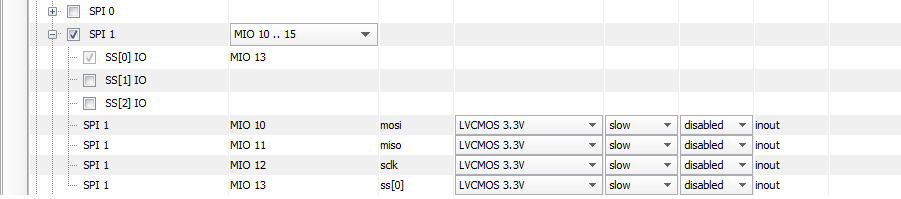
\includegraphics[width=1.00\textwidth]{picture/Pin_setup.png}
	\caption{Vivado SPI pinout}
	\label{fig:rfm12}
\end{figure}

The same Bitstream can be used for the Linux module and the Bare-metal program. The first attempt for loading the Bitstream was to start Linux and simply program the FPGA with the internal driver: \verb|cat bitstream.bit > /dev/xdevcfg|. This is working very easy and can be extended with the crontab program to program the FPGA after start-up. Therefore this simple line has to be added to crontab:\verb|@reboot cat /root/system_wrapper.bit > /dev/xdevcfg|. To configure crontab the following call can be used: \verb|crontab -e|\newline

\emph{But this is not working with the SPI}. While the System is booting it checks if the desired Hardware is available in the FPGA. So the OS thinks there is a SPI, but it is not in the FPGA. It just appears after the start-up. The Solution for this is to program the FPGA before the u-boot Bootloader loads the Linux in the RAM. Therefore the MicroZed Board has 2 Bootloader. The First Stage Bootloader can program the FPGA and after that he is loading the u-boot which is loading the Linux. The First Stage Bootloader can easily be created with the SDK of Xilinx. An step by step instruction can be fund on GitHub \url{https://github.com/SchoAr/RFM12_Linux/blob/master/FSBL/how_to_create_fslb.txt}\newline
Important is that the Board Support Package of the First stage Bootloader contains the SPI. Otherwise the programming might not work. The U-boot Image can be downloaded from Xilinx. A compiled version can also be found on GitHub. After compiling the Bootloader it is simply copied on the SD Card. 

\subsection{Device tree}

As described before the Device tree contains the hardware which is available via the Linux. The File which contains the Device tree can be found in the following directory:\newline\verb|./arch/arm/boot/dts/zynq-7000.dtsi|. In the predefined Device tree the SPI is not enabled. The SPI1 is simply enabled by deleting the "disable" status. The Following code shows this:

\begin{lstlisting}
spi1: spi@e0007000 {
					compatible = "xlnx,zynq-spi-r1p6";
          reg = <0xe0007000 0x1000>;
-         status = "disabled";   						//Delete this
          interrupt-parent = <&intc>;
          interrupts = <0 49 4>;
          clocks = <&clkc 26>, <&clkc 35>;
    }                                                                                                                           
\end{lstlisting}

Now we need to add in the settings the SPI Configuration this is done in the following file:\newline\verb| ./arch/arm/boot/dts/zynq-zed.dts|. Here are the parameters for the devices saved. Here the SPI1 has to be added to use it for the Driver. The following listing shows the code,which has to be added:
\begin{lstlisting}
+&spi1 {
+        status = "okay";
+        num-cs = <4>;
+        is-decoded-cs = <0>;
+};
\end{lstlisting}

It is also possible to add a specific device to the device tree which can then be used in user space. The following listing shoes this example. If this is applied a SPI master device will appear in /dev. With a simple echo command it is possible to send Data. This is good practice if it is necessary to test the SPI without writing a Module. This has been done to check if the first stage Bootloader loaded successful the Bitstream in the FPGA.

\begin{lstlisting}
&spi1 {
       status = "okay";
       num-cs = <4>;
       is-decoded-cs = <0>;
       device@2 {
                compatible = "spidev";
                reg = <0>;
                spi-max-frequency = <500000>;
                };            
};
\end{lstlisting}



\emptydoublepage
\chapter{Developing the Module}

A good overview of module development can be found in this book: \url{http://lwn.net/Kernel/LDD3/}\newline

This Chapter describes the development of the Module. The Documentation is described for the commit with the number \verb|e60cffe5ad3cda37924a5ba57fd7f89476cb4fc6|. The latest version can be found on GitHub with the link:\url{https://github.com/SchoAr/RFM12_Linux/tree/master/Modules}.\newline
The Compiler for this module is not a standard GCC. Because The Compiled output has to be working on a ARM processor and not on an Intel. Therefore a Cross Compiler has to be used. With that it is possible to compile on a Intel machine code for a ARM processor. The Instructions how to get the cross compiler running can be found here \url{https://github.com/dasGringuen/MicroZedKernel/blob/master/02-toolchain.txt}
For the Compilation of the Driver a special makefile was taken. It contains the path to the Kernel Sources, and the IP address of the Target. With the command \verb|make| the Driver is compiling. With the command \verb|make install| the compiled Driver is copied to the target device. \newline
All the Components of the Driver are saved in one File, cause they all belong to the driver of the RFM12. 

\subsection{Loading and unloading the module}

Before we discuss the basics of a module, we discuss the basic System calls for the module Development. They are very important for the Debugging and the working with the module. 
The first System call is \verb|insmod|, with this it is possible to load the module into the Kernel. For example with \verb|insmod RFM12| the module of the RFM12 is loaded into the Kernel. Before we can load a newer version of the module into the Kernel we have to remove the older one. This is done with the System calls \verb|rmmod|. Very helpful for the debugging is the System calls \verb|lsmod|. This shows the running modules, and also the Memory needed from each. For Debugging the most impotent is \verb|dmesg|. This shows the Messages which are printed with the Kernel print function. With the function \verb|printk|, every Debug print is realised. \newline
For a easy use of the above described calls a script is available. This script unloads first the module, and after that the older Kernel prints are deleted. After that the Script loads the new module and shows how much Memory is needed. The Script is also on GitHub :\url{https://github.com/SchoAr/RFM12_Linux/blob/master/module_run}.\newline

The most simple Driver has just a method which is called when he is loaded, and one which is called when he is unloaded. Here is an example of this: \url
{https://github.com/dasGringuen/MicroZedKernel/blob/master/src/hello_world/hello.c}. It can also be found in the used repository in one of the first commits. Important is that the functions are simply declared and the Kernel knows that he has to call this functions via the following macros: 

\begin{lstlisting}
module_init(RFM_init);
module_exit(RFM_exit);
\end{lstlisting}

With this Macros the Module can give also other Information to the Kernel like the following:

\begin{lstlisting}
MODULE_AUTHOR("Schoenlieb");
MODULE_DESCRIPTION("A Char Driver for the RFM12 Radio Transceiver");
MODULE_LICENSE("GPL");                                                                                                                        
\end{lstlisting}

In the function RFM12\_init the whole driver gets initialized. This means that after the end of this function everything has to be ready to use the Device. The first thing which is done in the module is to Initialise the GPIO. This is done with a function call. This function will be described in the GPIO section of the module. Important is that the return value has to be checked if that woks. After that the SPI is Initialized. Here also the return value is checked if this is working. The problem in this version of the module is, that if the SPI initialisation fails the function is finished, and the GPIO is still allocated. This can cause mayor problems, because the de-initialisation can fail. Cause it try s to de-initialise something which don’t exist. This can cause the last possibility to reset the Device. This is not a option in the final module. \newline
The right way to do an error handling is shown by the registration of the file operations. If they fail the GPIO is freed and the start position is nearly reached. Nearly reached because the SPI is not freed. The state of the module shows that the SPI is not fully integrated yet. Now that the Hardware is Initialized, the RFM12 can be Initialized. The Driver does not support a other configuration of the RFM12 yet. This will be implemented in the future. For Debugging reasons a print indicates that the Initialisation was successful. \newline

If the module gets unloaded, it has to de-initialise everything. if this function is not working as expected the loading of the module wont work any more and the device has to be resetted. This indicates that a exit method is as important as the initialize method. The order of the freeing is not important but everything has to be considered. Happily at the developing process it is noticed if the exit method is not working correctly. Cause every time a newer version is tested the older driver has to be unloaded. If he cant allocate all resources any more the exit method should be checked.  

\subsection{Read and Write Functions}

The read and write functions are very important, because they are used for sending and receiving data with the RFM12. There is a tutorial via this link: \url{http://www.codeproject.com/Articles/112474/A-Simple-Driver-for-Linux-OS}. The RFM12 Driver which has the read write operations implemented, without the SPI and the RFM12 functions can be found via this link: \url{https://github.com/SchoAr/RFM12_Linux/blob/66c55b2286c8d3eae915cd521587cd6160c13055/Modules/RFM12.c}. On GitHub also exists a test program which interacts with the RFM12 module. It can be found via this link and will be discussed later in this Chapter: \url{https://github.com/SchoAr/RFM12_Linux/blob/7d31dd367e1de8eefa65ea900e642b0e6b27f790/RFM12_test.c}.\newline This program has been changed, to match the Bare-metal main loop implementation. But this version shows the working of the read and write functions. \newline

The read function should simply return a "Hello World" string to indicate that the read method is working. This is done with this function: 
\begin{lstlisting}   
static const char *id = "Hello World";
                                                                                                                    
static ssize_t read(struct file *file, char __user *buf, size_t count,loff_t *ppos)
{
		printk(KERN_INFO "Read is called !\n");
		return simple_read_from_buffer(buf, count, ppos, id, strlen(id));
}
\end{lstlisting}

The Prototype of this function is given. It simply copies the values form the buf to the given buffer from the function. So it is simply separating the memory of the Kernel to the memory of the user space. This function can also be used with the build in function \verb|cat|. \newline

The write function is similar to the read it is coping the received data in an internal buffer. In this case the buffer is just used to indicate that we received something and print it to the kernel log. 

\begin{lstlisting}
  static ssize_t write(struct file *file, const char __user *buf,size_t count, loff_t *ppos)
{
		char temp[32] = {};
		printk(KERN_INFO "write is called !\n");
		simple_write_to_buffer(temp, sizeof(temp), ppos, buf, count);
		printk(KERN_INFO "write value = %s \n",temp);
		return 0;
}                                                                                                                        
\end{lstlisting}

This function is not working with the echo command because the echo command is not indicating how much data is passed to this function.The function simply freezes because it is waiting for a infinite amount of data and receives only a finite number. In a further state of the driver the length should be indicated by the length of the passed array. Never the less this function is working with the test program and has also be changed for the sending functionality of the RFM12. \newline

Now when we have this functions we need to tell the Kernel that they exist and what it should do with it. This is done via this 2 structs. 

\begin{lstlisting}
  static const struct file_operations fops = {
		.owner = THIS_MODULE,
		.read = read,
		.write = write,
	};
	
	static struct miscdevice eud_dev = {
		.minor = MISC_DYNAMIC_MINOR,
		.name = "RFM12_RW",
		.fops = &fops
	};                                                                                                                       
\end{lstlisting}

The first struct indicates which operations are available and saves the pointer to this functions. There are more functions which can be assigned. In a Future state of the module the open and close method can be used to indicate that the receiving is possible or not. \newline
The second struct handles the registration of the module. The minor number is assigned dynamically by the operating System and the module does not care about it. But it is necessary for the numbering of the module. Important is the name, it indicates which name will be displayed to the user. The name will be found at "/dev/RFM12\_RW". \newline

The first step in testing this program is to open the RFM12\_RW device. after that the write is simply tested with this line \verb| write(fp,"Hallo", 5);|. This will be visible in the Kernel log. The read function is looking similar, it just gives a struct which will receive the data. The call is as followed: \verb| ret = read(fp,&str,10);|. This function will receive the hello world string. After the operations it is important to close the file again, otherwise it cant be opened any more. 

\subsection{GPIO Operation}

For accessing hardware the GPIO is normally the first choice. Also in this project the GPIO was the first choice. Also it will be needed for the 3 LEDs and the Interrupt. There exists an tutorial which describes how to access the GPIOS and how to register an Interrupt on them. It can be found via this link: \url{https://github.com/wendlers/rpi-kmod-samples/blob/master/modules/kmod-gpio_inpirq/gpiomod_inpirq.c}. All the needed defines can be found in this file : RFM12\_config.h.\newline
The Version of the RFM12 at which the GPIO Interrupt toggles an LED can be found via this link: \url{https://github.com/SchoAr/RFM12_Linux/blob/interrupt_work/Modules/RFM12.c}.\newline

Before we can initialize the GPIOs we have to define it somewhere. This is done via the following struct: 

\begin{lstlisting}
	static struct gpio leds[] = {
		{ ON_LED, GPIOF_OUT_INIT_HIGH, "ON" },
		{ RX_LED, GPIOF_OUT_INIT_HIGH, "RX" },
		{ TX_LED, GPIOF_OUT_INIT_HIGH, "TX" },
	};                                                                                                                
\end{lstlisting}

The defines of *\_LED can be found in the RFM12\_config.h file, and simply describes the Pin at which the LEDs are connected.\newline Now the function \verb|ret = gpio_request_array(leds, ARRAY_SIZE(leds));| is used to request the GPIOs. After that the Module can use the GPIOs very easy.\newline With the function \verb|gpio_set_value(leds[i].gpio,1);| the LED is turned on. To turn it of the 1 has to be replaced with a 0.\newline 

The Interrupt input is defined via a array. Also the input IRQs need to be declared declaration. The following listing shows the definition: 

\begin{lstlisting}
	static struct gpio input[] = {
		{ INPUTPIN, GPIOF_IN, "INPUT" },
	};
	
	static int input_irqs[] = { -1 };
\end{lstlisting}

Before we can declare the Interrupt we also need to request the GPIO. After that we can use this function: \verb| ret = gpio_to_irq(input[0].gpio);| to get a IRQ from a GPIO. This is saved in the input\_irq array. Now the following function call defines the IRQ: 

\begin{lstlisting}
 ret = request_irq(input_irqs[0], input_ISR, IRQF_TRIGGER_RISING | IRQF_DISABLED, "gpiomod#input1", NULL);
\end{lstlisting}

With this function call we define every parameter of the Interrupt. The Input ISR is passed and called when then interrupt is triggered. The Trigger is a Rising edge. This is changed in later versions of the module. Now we have the same Interrupt behaviour as in the Bare-metal program.\newline

In GPIO Initialization is a good example how good error management is done. Normally it is not used to work in C with labels, but in this case it is very useful. If the request of the Interrupt fails the LEDs are freed. If the initialisation of the Interrupt fails, all GPIOs are freed. If this function fails everything is as before.
 
\subsection{SPI}

The connection via the SPI Interface is more difficult than the usage of a GPIO. Here is no explanation of the SPI Interface, because it should be known at this point. A Tutorial for the SPI module can be found via this link: \url{http://wenku.baidu.com/view/ab20084269eae009581bec37} . It describes the basic function of the programming. Another Resource for information can be found via this link: \url{https://www.kernel.org/doc/Documentation/spi/spi-summary}.\newline

Very important is to test the SPI with a spidev driver, described in the device Tree section. After the spidev is removed we can seek for the number of the SPI controller. It can be found in this directory: \verb| /sys/class/spi_master|. There are 2 numbers spi0 and spi32766. To try spi0 will not work very well cause it is the SPI for the SD Card and is already in use. Therefore we need the other SPI. Now we can create a spi\_driver struct via the following struct. The 2 functions are required for the driver to indicate the load and unload for the SPI driver.

\begin{lstlisting}
	static int RFM12_probe(struct spi_device *spi_devicef)
	{
		spi_device = spi_devicef;
		return 0;
	}
	
	static int RFM12_remove(struct spi_device *spi_devicef)
	{
		spi_device = NULL;
		return 0;
	}
	
	static struct spi_driver RFM12_driver = {
		.driver = {
			.name = "RFM12_spi",
			.owner = THIS_MODULE,
		},
		.probe = RFM12_probe,
		.remove = RFM12_remove,
	};
\end{lstlisting}

Now it is necessary to request the SPI master. This is done with the following function: \verb|spi_master = spi_busnum_to_master(SPI_BUS);|. Here the SPI number is needed, which was looked up before. Now that we have a master device which controls the bus we can access a spi\_device. The Function which allocates this device is the following:\newline
\verb|spi_device = spi_alloc_device(spi_master);|. This device is the most important part for the SPI communication, because it is the abstraction of the RFM12 on the SPI bus. Now the device for the RFM12 can be configured with this parameters: 

\begin{lstlisting}
	spi_device->chip_select = SPI_BUS_CS0; 		//0

	spi_device->max_speed_hz = SPI_BUS_SPEED; //200000
	spi_device->mode = SPI_MODE_0;						
	spi_device->bits_per_word = 8;
	spi_device->irq = -1;
	spi_device->controller_state = NULL;
	spi_device->controller_data = NULL;                                                                                                                         
\end{lstlisting}

The Chip select is 0 as defined in the Vivado and the Bus speed is fixed with max 200kHz. With the SPI\_MODE\_0 the normal clock parameter are defined. The values for this can be found in the spi.h in the Kernel sources. In this case the clock is active high an has no phase. Now the Device can be registered to the master via the following function:\newline \verb| status = spi_add_device(spi_device);|.\newline

There are 2 functions for the sending via the SPI. The first is:\verb|spi_sync(spi_device, &msg);|. This function waits until the sending is finished. Because waiting is not allowed, and it will be punished with a total system failure, there is another function. This function returns after the sending is started, and a callback indicates that the sending has finished. The function call of the sending as as followed: \verb|spi_async(spi_device, &msg)|.\newline

To send data via the SPI a spi\_transfer struct has to be created. It holds the Buffers for the sending and receiving. in the RFM12.c exists a function which creates a transfer struct. The function is as followed: 

\begin{lstlisting}

struct spi_transfer rfm12_make_spi_transfer(uint16_t cmd, u8* tx_buf, u8* rx_buf)
{
	struct spi_transfer tr = {
		.tx_buf = tx_buf,
		.rx_buf = rx_buf,
		.len = 2,
	};
	tx_buf[0] = (cmd >> 8) & 0xff;
	tx_buf[1] = cmd & 0xff;
	return tr;
}                                                                                                                          
\end{lstlisting}
  
This function receives a u16 which is then put into the tx buffer. Receiving is not necessary in this case. After this struct is created it can be added to the message. The message has to be initialised before. The add function is the following: \verb|spi_message_add_tail(&tr1, &msg);|.

\subsection{Implementation of the RFM12}

The Initialisation of the RFM12 takes the same Parameter as the Bare-Metal program. It sends also the same commands to the RFM12, but the sending is done in an other way. The first attempt to Initialise the RFM12 was to create a message with 1 transmission and send it synchronously. This is working, but the time for the Initialisation function to be finished is enormous. This is not very useful in a system if the module needs to load 3 seconds. In a other project the module Initialisation is done in an other way. The code for this can be found with this link: \url{https://github.com/gkaindl/rfm12b-linux/blob/master/rfm12b.c}. \newline
Not every message is send with just one transmission. The transmissions are send with just 2 messages. The following listing shows this concept for the first part of the initialisation. 

\begin{lstlisting}
	spi_message_init(&msg);
	
	tr1 = rfm12_make_spi_transfer(RF_SLEEP_MODE,tx_buf+2,NULL); // DC (disable clk pin), enable lbd
	tr1.cs_change = 1;
	spi_message_add_tail(&tr1, &msg);
	
	tr2 = rfm12_make_spi_transfer(RF_TXREG_WRITE,tx_buf+4,NULL); // in case we're still in OOK mode
	tr2.cs_change = 1;
	spi_message_add_tail(&tr2, &msg); 
		
	err = spi_sync(spi_device, &msg);
	if (err){
		printk(KERN_INFO "Error sending 2 SPI Message %d!\n",err);
	}
	msleep(100);
                                                                                                                          
\end{lstlisting}

For the sending method the write method has to be changed. It is simply calling the SendStart function which is already known from the Bare-metal program. One difference is here that the coping of the data is done in the SendStart function, and cause twice coping is not needed this is not needed in the write function. The following listing shows how it is done. 

\begin{lstlisting}
static ssize_t write(struct file *file, const char __user *buf,size_t count, loff_t *ppos)
{
	/*The copieng of the user buffer is done in SendStart*/
	SendStart(SERVER_MBED_NODE, buf,count, 0,0);
	return 0;
}
\end{lstlisting}

At this point the read function is not created for the RFM12. \newline

At this point of the development process the Interrupt is not working properly. It is possible to send Data in the Interrupt, but the RFM12 is not working with them. The main problem is that the Interrupt is doing the sending. This was a first attempt taken from the Bare-metal program but it is not sufficient for a Linux module. \newline

The Idea now is to let a tasklet be scheduled in the Interrupt. This is then Synchronous to the other processes. This allows the usage of the spi\_synchronus function which is much easier to handle. an example for a tasklet can be found cia this link : \url{http://blogsmayan.blogspot.co.at/p/programming-interrupts-in-raspberry-pi.html}
\emptydoublepage
%\bibliography{Literatur}

% place all floats and create label on last page
\FloatBarrier\label{end-of-document}
\end{document}

